\documentclass[../../dissertation.tex]{subfiles}
\begin{document}

Consider the example of a quantum walker on a discretely numbered cycle. It was seen that the evolution operator associated with such a system is, as was defined in equation \ref{eq:coinedUnmarkedOperator}
\begin{equation}
	   U = S(C\otimes I), 
           \label{eq:coinedUnmarkedOperatorQiskit}
\end{equation}
%TODO: Decidir se menciono as equacoes do shift e da coin.
where $S$ is a shift operator, defined in equation \ref{eq:coinedShiftOperator} as 
\begin{equation}
          S = \ket{0}\bra{0} \otimes \sum_{x=-\infty}^{x=\infty} \ket{x+1}\bra{x} + \ket{1}\bra{1}\otimes \sum_{x=-\infty}^{x=\infty} \ket{x-1}\bra{x},
\end{equation} 
that increments or decrements the position of the walker according to the coin operator $C$.\par
%TODO: Reescrever prox paragrafo.
Previously, this system was simulated in Python by implenting it's equations. Now, the focus is to study a quantum circuit based on the work presented by \cite{douglaswang07}. This approach relies on multi-controlled CNOT gates in order to shift the state of the walker by $+1$ or $-1$, each with a probability associated with the chosen coin, as can be seen in figure \ref{fig:douglasWangShift}. 

%TODO: Decidir se ficam 3 pontos verticais.
%TODO: Substituir todas as minipages por subfigures.
\begin{figure}[!htb]
	\centering
	\begin{subfigure}[t]{0.40\textwidth}
        \[ \Qcircuit @C=1em @R=.7em {& \targ    & \qw      & \qw      & \qw      & \qw \\
        			  & 	     & 	        &          &          &  . \\
        			  & 	     & 	        &          &          &  . \\
        			  & 	     & 	        &          &          &  . \\
        			  & \ctrl{-4} & \targ   & \qw      & \qw      & \qw \\
        			  & \ctrl{-1} & \ctrl{-1} & \targ    & \qw      & \qw\\ 
        			  & \ctrl{-1} & \ctrl{-1} & \ctrl{-1} & \qw      & \qw
			  } \]
	\caption{Douglas wang increment}
	\label{fig:coinedIncrement}
	\end{subfigure}
	\begin{subfigure}[t]{0.40\textwidth}
        \[ \Qcircuit @C=1em @R=.7em {& \targ    & \qw      & \qw      & \qw      & \qw \\
        			  & 	     & 	        &          &          &  . \\
        			  & 	     & 	        &          &          &  . \\
        			  & 	     & 	        &          &          &  . \\
        			  & \ctrlo{-4} & \targ   & \qw      & \qw      & \qw \\
        			  & \ctrlo{-1} & \ctrlo{-1} & \targ    & \qw      & \qw\\ 
        			  & \ctrlo{-1} & \ctrlo{-1} & \ctrlo{-1} & \qw      & \qw
			  } \]
	\centering
	\caption{Douglas wang Decrement}
	\label{fig:coinedDecrement}
	\end{subfigure}
	\caption{Douglas wang shift operator}
	\label{fig:douglasWangShift}
\end{figure}

%TODO: Melhorar o paragrafo seguinte
The generalized CNOT gates act on the node states as a cyclic permutator, where each node is mapped to an adjacent state. This can be seen as the walker moving left or right, in the uni-dimensional graph example.\par

%TODO: Descobrir como separar a moeda do resto do circuito. Adicionar node e subnode?
%TODO: Fazer um circuito para N=3 ou N=4 e por os resultados da simulacao com esse numero. 
%TODO: Resize da figura?
\begin{figure}[!h]
	\[ \Qcircuit @C=1em @R=0em { &\qw & \multigate{4}{incr} &  \multigate{4}{decr} & \qw \\
				     &\qw & \ghost{incr} & \ghost{decr} & \qw \\
               			     &\qw & \ghost{incr} & \ghost{decr} & \qw \\
            			     &\qw & \ghost{incr} & \ghost{decr} & \qw \\
            			     &\qw & \ghost{incr} & \ghost{decr} & \qw \\ 
				     &    &              &              &     \\
				     &    &              &              &     \\
				     &    &              &              &     \\
				     &\gate{H} & \ctrl{-2} & \ctrlo{-2} & \qw 
		          } \]
	\centering
	\caption{Douglas wang coined quantum walk circuit}
	\label{fig:coinedCircuit}
\end{figure}

The coin operator will simply be a Hadamard gate acting on a single qubit. For a graph with $16$ nodes, for example, $4$ qubits are required to encode each node and an extra qubit for the coin. The circuit will then be as shown in figure \ref{fig:coinedCircuit}. Note that this circuit limits the number of graph nodes to powers of $2$, and an arbitrary implementation of $2^n$ nodes requires $n+1$ qubits.
%TODO: Decidir como falar sobre como implementar nos que nao sao potencias de 2. Deverei mencionar a figura do artigo do doulgas wang?
%TODO: Descobrir uma source diferente para o gray code ordering. Nielsen chuang.
However, it is possible to have any number of nodes, given that the proper correction is made as can be seen in \cite{douglaswang07}. The method used was \textit{Gray Code Ordering} proposed by \cite{alexslepoy06}, whereby a certain arrangement of CNOT gates results in control states only differing by a single bit.\par
In order to run this circuit on a real quantum computer using Qiskit, one must first find a way of creating generalized CNOT gates, since it is not available in the base package. One approach to this problem is to decompose an arbitrarily controlled CNOT gate into elementary gates, as was done by \cite{barenco95}. In this context, the main idea is that for any unitary operator $U$, there exists operators such that 
\begin{equation}
	U = \phi AXBXC,
\end{equation}
where $ABC=I$, $X$ is the Pauli-X and $\phi$ is a phase operator described by $\phi=e^{i\delta} \times I$.\par
\begin{figure}[!h]
	\[ \Qcircuit @C=1em @R=1em { & \ctrl{2} & \qw & \\
			&\ctrl{1} &\qw & = &  \\
			&\targ & \qw &
		}
		 \Qcircuit @C=1em @R=1em { &\ctrl{2} & \qw  & \qw  & \ctrl{2} & \qw & \ctrl{2} & \qw & \qw\\
				     &\ctrl{1} & \ctrl{1} & \ctrl{1} & \qw & \ctrl{1} & \qw & \ctrl{1} & \qw\\ 
				     &\gate{\phi(\frac{\pi}{2})} & \gate{R_z(\frac{\pi}{2})}  & \gate{R_y(\frac{\pi}{2})} & \targ & \gate{R_y(-\frac{\pi}{2})} & \targ &\gate{R_z(-\frac{\pi}{2})} & \qw 
		          } \]
	\centering
	\caption{Toffoli decomposition}
	\label{fig:toffoliDecompCircuit}
\end{figure}
In order to understand this method, a good first example is the Toffoli gate, as is shown in figure \ref{fig:toffoliDecompCircuit}. 
%TODO: Explicar a decomposicao da cnot? Ver a dissertacao.
%TODO: Target nao fica alinhado com as unitarias.
%TODO: Reescrever isto. A primeira rotacao nao e Rz.
The first rotation in the circuit is defined by the $R_z$ matrix 
\begin{equation}
	R_z(\theta) = \begin{pmatrix}
		e^{i\frac{\phi}{2}} & 0 \\
		0 & e^{i\frac{\phi}{2}}
	\end{pmatrix},
\end{equation}
where $\theta = \frac{\pi}{2}$. Secondly, the $R_y$ rotation is
\begin{equation}
	R_y(\phi) = \begin{pmatrix}
			cos(\frac{\theta}{2}) & -sin(\frac{\theta}{2}) \\
			sin(\frac{\theta}{2}) & cos(\frac{\theta}{2})
		 \end{pmatrix},
\end{equation}
and $\phi = \frac{\pi}{2}$. The following rotations are simply $R_z^\dagger$ and $R_y^\dagger$. Lastly, the phase operator $\phi$ is 
\begin{equation}
	\phi(\delta) = \begin{pmatrix}
		e^{i\delta} & 0 \\
		0 & e^{i\delta}
		 \end{pmatrix}
\end{equation}
where $\delta = -\frac{\pi}{2}$. This phase correction is considered because otherwise
\begin{equation}
	R_z(\frac{\pi}{2})R_y(\frac{\pi}{2})XR_y(-\frac{\pi}{2})XR_z(-\frac{\pi}{2}) = 
	\begin{pmatrix}
		0 & -i \\
		-i & 0
		 \end{pmatrix} \neq X.
\end{equation}
Introducing the phase correction results in
\begin{equation}
	\phi(\frac{\pi}{2}) 
	\begin{pmatrix}
		0 & -i \\
		-i & 0
		 \end{pmatrix} =  
	\begin{pmatrix}
		i & 0 \\
		0 & i
		 \end{pmatrix}   
	\begin{pmatrix}
		0 & -i \\
		-i & 0
		 \end{pmatrix} =   
	\begin{pmatrix}
		0 & 1 \\
		1 & 0
		 \end{pmatrix} = X  
\end{equation}
%TODO: Rever esta frase e tentar expandir um bocado.
However, since this is a global phase, it won't be included since it has no effect on the result of the measurement.\par
%TODO: Rever parte do "generalised inverter gates"
A more generalized version of this method can be seen in figure \ref{fig:generalDecompCircuit}. Each individual generalized CNOT gate in this circuit can be expanded as was done for the Toffoli gate example, stopping once the generalised inverter gates are simply Toffoli gates.

\begin{figure}[!h]
	\[ \Qcircuit @C=1em @R=1em { & \ctrl{5} & \qw & \\
			&\ctrl{4} &\qw & = &  \\
			&         & .  &   &  \\
			&         & .  &   &  \\
			&         & .  &   &  \\
			&\ctrl{1} &\qw & = &  \\
			&\gate{U} & \qw &  &
		}
			\Qcircuit @C=1em @R=1em { 
				     &\ctrl{5} & \qw  & \ctrl{6} & \qw & \ctrl{6} & \qw &  \qw\\
				     &\ctrl{4} & \qw & \ctrl{5} & \qw & \ctrl{5} & \qw &  \qw\\ 			
				     &         & .  &   & . &  & . \\
				     &         & .  &   & . &  & . \\
				     &         & .  &   & . &  & . \\
				     &\ctrl{1} & \ctrl{1}  & \qw & \ctrl{1} & \qw &\ctrl{1} & \qw \\				     &\gate{\phi} & \gate{A}  & \targ & \gate{B} & \targ &\gate{C} & \qw 
		          } \]
	\centering
	\caption{General decomposition}
	\label{fig:generalDecompCircuit}
\end{figure}
This was the chosen method because it provides a way of implementing arbitrarily controlled CNOT gates without the use of ancillary qubits, which are a scarce resource.\par

\begin{figure}[!h]
	\centering
	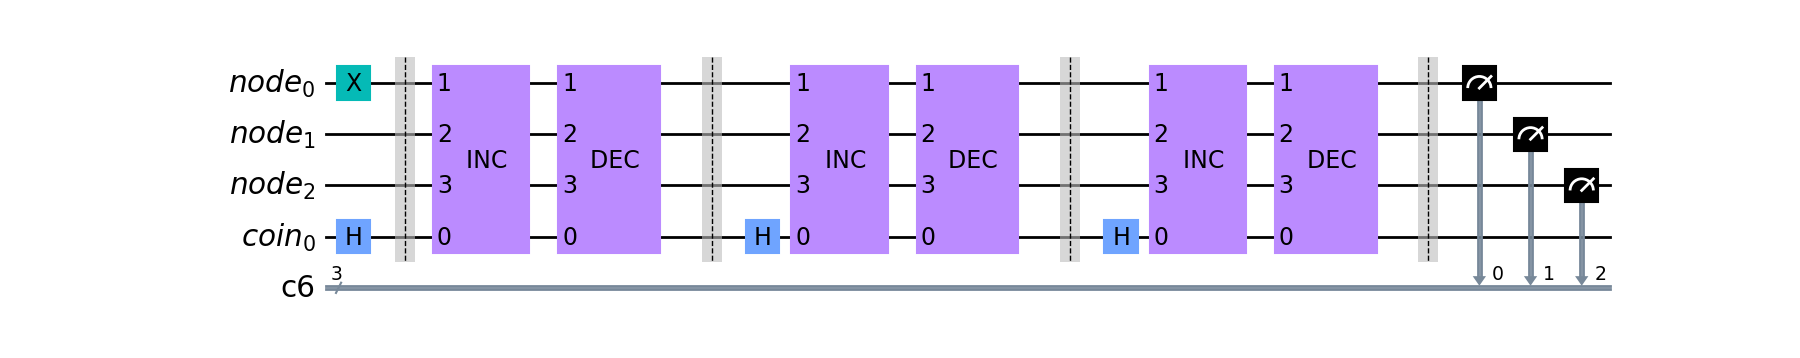
\includegraphics[scale=0.35]{img/Qiskit/CoinedQuantumWalk/Circuits/circCoinedQW_N3_S3.png}
	\caption{Temp} 
	\label{fig:coinedQWCircuitQistkit}
\end{figure}

This circuit was implemented in Qiskit, as can be seen in figure \ref{fig:coinedQWCircuitQistkit}. In this example, the increment and decrement sequence was applied three times on a graph of size $2^3 =8$ nodes. The starting position of the walker was set to $\Psi(0) = \ket{4}$ and the Hadamard coin was used. The first block after the barrier is the sequence of operations that will increment the state of the walker, as is shown in figure \ref{fig:incrCircuitQistkit}. The circuit is simply the CNOT decomposition of figure \ref{fig:generalDecompCircuit} applied to the increment circuit of figure \ref{fig:coinedIncrement} for the $N=4$, qubit case.
\begin{figure}[!h]
	\centering
	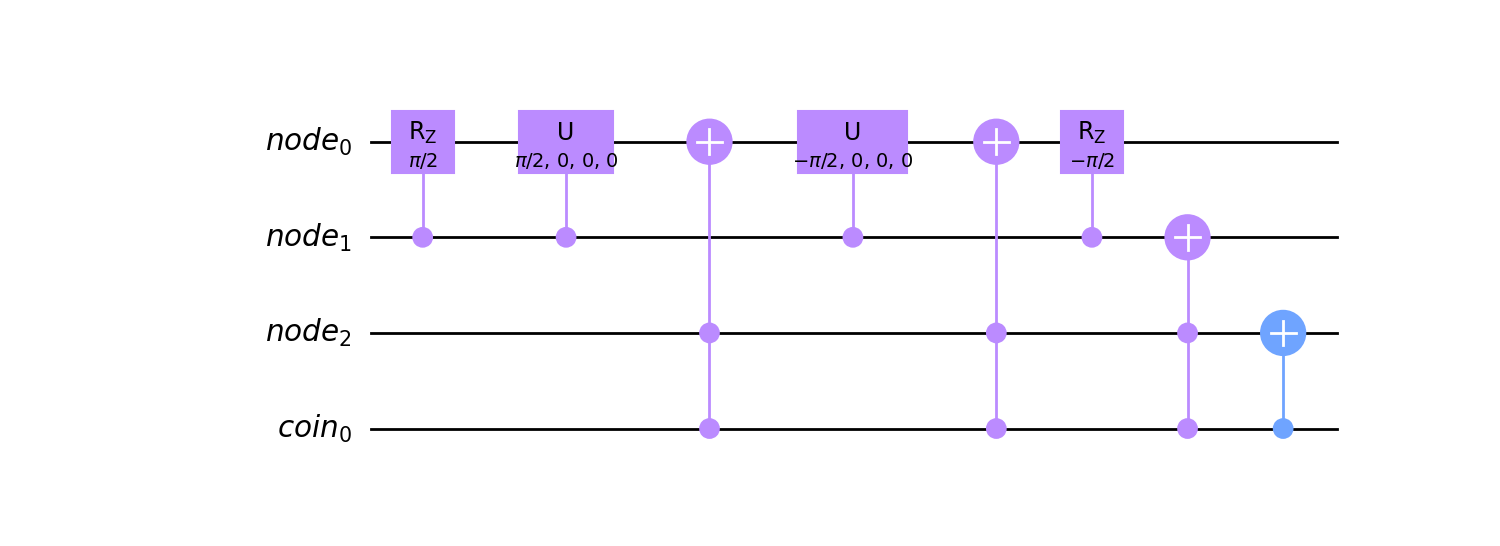
\includegraphics[scale=0.35]{img/Qiskit/CoinedQuantumWalk/Circuits/circIncr_N3_S3.png}
	\caption{Temp} 
	\label{fig:incrCircuitQistkit}
\end{figure}
The following block represents the decrement of the state of the walker, which is just an increment block with it's controls negated as is shown in figure \ref{fig:decrCircuitQistkit}. The rest of the circuit is just the repetition of these operations as a function of the number of time steps required.

\begin{figure}[!h]
	\centering
	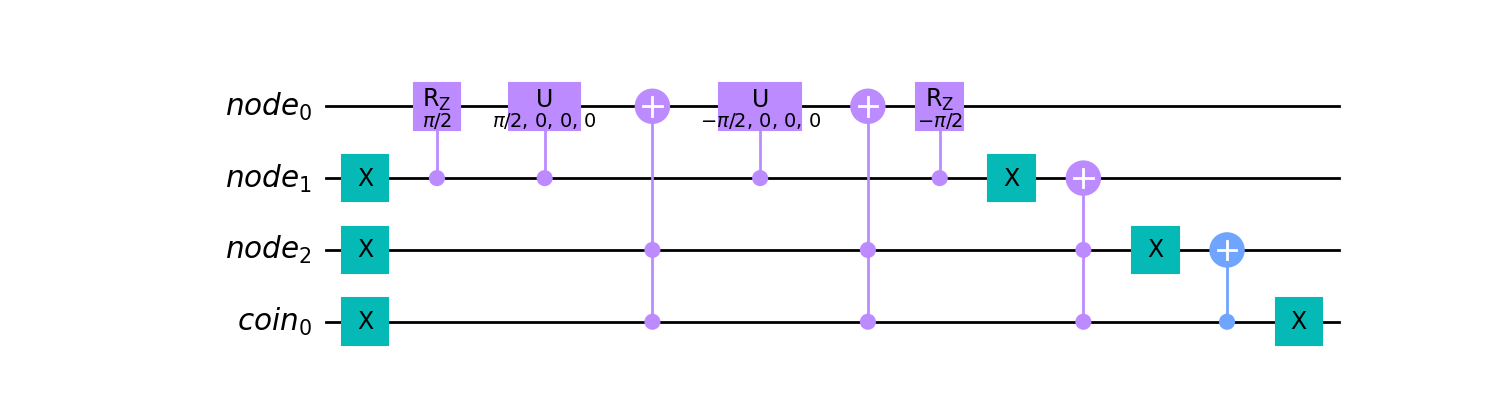
\includegraphics[scale=0.35]{img/Qiskit/CoinedQuantumWalk/Circuits/circDecr_N3_S3.png}
	\caption{Temp} 
	\label{fig:decrCircuitQistkit}
\end{figure}
Lastly, the circuit is measured and the results can be seen in figure \ref{fig:coinedQWQiskitDist}.These results can be verified by calculating the time evolution of the wave function associated with the system
\begin{gather}
	\ket{\Psi(0)} = \ket{4}\\
	\ket{\Psi(1)} = \frac{\ket{0}\ket{x=3}+\ket{1}\ket{x=5}}{\sqrt{2}}\label{eq:10} \\
	\ket{\Psi(2)} = \frac{\ket{0}\ket{x=2}+\ket{1}\ket{x=4}+\ket{0}\ket{x=4}-\ket{1}\ket{x=6}}{2}\\ \label{eq:11}
	\ket{\Psi(3)} = \frac{\ket{1}\ket{x=1}-\ket{0}\ket{x=3}+2(\ket{0}+\ket{1})\ket{x=5}+\ket{0}\ket{x=7}}{2\sqrt{2}}.\label{eq:12}
\end{gather}
Taking the modulus squared of the amplitudes associated with the states, confirms that the probability distribution presented in figure \ref{fig:coinedQWQiskitDist} is correct. 
\begin{figure}[!h]
	\centering
	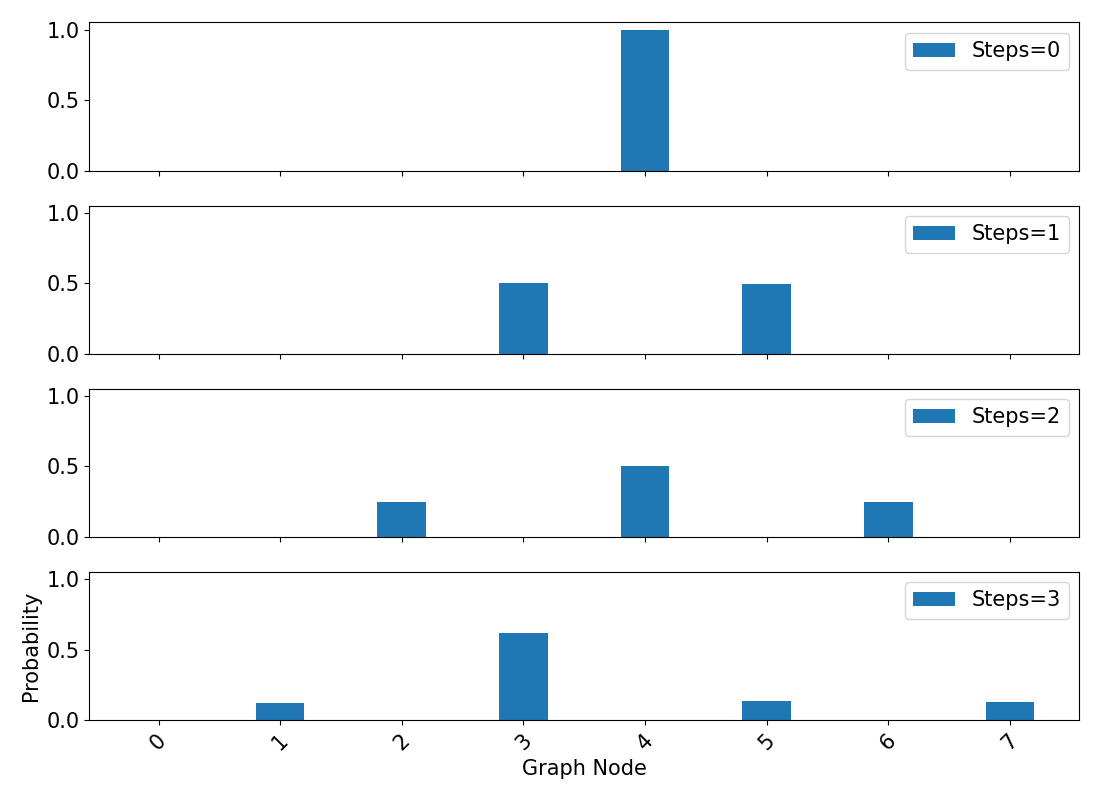
\includegraphics[scale=0.40]{img/Qiskit/CoinedQuantumWalk/CoinedQW_N3_S0123.png}
	\caption{Temp} 
	\label{fig:coinedQWQiskitDist}
\end{figure}
%TODO: Pensar numa conclusao para esta seccao. Talvez por N=5? Explicar cada passo de N=5 nao e fazivel.

\end{document}
